% This file was created by tikzplotlib v0.9.8.
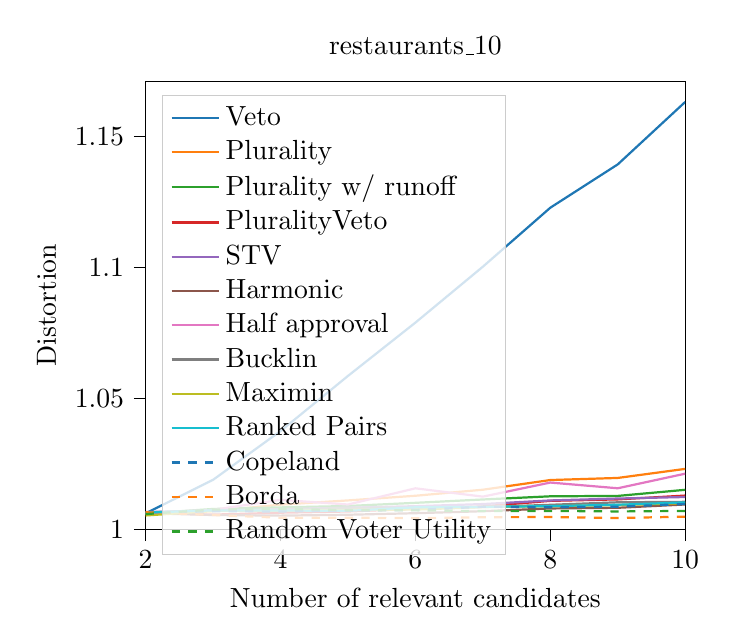
\begin{tikzpicture}

\definecolor{color0}{rgb}{0.12156862745098,0.466666666666667,0.705882352941177}
\definecolor{color1}{rgb}{1,0.498039215686275,0.0549019607843137}
\definecolor{color2}{rgb}{0.172549019607843,0.627450980392157,0.172549019607843}
\definecolor{color3}{rgb}{0.83921568627451,0.152941176470588,0.156862745098039}
\definecolor{color4}{rgb}{0.580392156862745,0.403921568627451,0.741176470588235}
\definecolor{color5}{rgb}{0.549019607843137,0.337254901960784,0.294117647058824}
\definecolor{color6}{rgb}{0.890196078431372,0.466666666666667,0.76078431372549}
\definecolor{color7}{rgb}{0.737254901960784,0.741176470588235,0.133333333333333}
\definecolor{color8}{rgb}{0.0901960784313725,0.745098039215686,0.811764705882353}

\begin{axis}[
legend cell align={left},
legend style={
  fill opacity=0.8,
  draw opacity=1,
  text opacity=1,
  at={(0.03,0.97)},
  anchor=north west,
  draw=white!80!black
},
tick align=outside,
tick pos=left,
title={restaurants\_10},
x grid style={white!69.0196078431373!black},
xlabel={Number of relevant candidates},
xmin=2, xmax=10,
xtick style={color=black},
y grid style={white!69.0196078431373!black},
ylabel={Distortion},
ymin=1, ymax=1.17103579894585,
ytick style={color=black}
]
\addplot [thick, color0]
table {%
2 1.00611822577974
3 1.01892136136559
4 1.03751652964445
5 1.05855934822612
6 1.07890106979938
7 1.10023401607912
8 1.12274010720627
9 1.13926857246888
10 1.163095638501
};
\addlegendentry{Veto}
\addplot [thick, color1]
table {%
2 1.00590317642056
3 1.00697946126373
4 1.00945467958997
5 1.01106894529547
6 1.01284809071051
7 1.01514926695142
8 1.01884591002291
9 1.01964211238776
10 1.0231022770988
};
\addlegendentry{Plurality}
\addplot [thick, color2]
table {%
2 1.00604964264549
3 1.00781029473048
4 1.00840994665999
5 1.00893725037744
6 1.0101485176227
7 1.01142615607069
8 1.01263763509085
9 1.01278878514596
10 1.01511416641361
};
\addlegendentry{Plurality w/ runoff}
\addplot [thick, color3]
table {%
2 1.00637330207936
3 1.00565790706972
4 1.00638061709435
5 1.00683984493299
6 1.00786127799263
7 1.00879269902724
8 1.01089923454167
9 1.01145528421935
10 1.01292110072059
};
\addlegendentry{PluralityVeto}
\addplot [thick, color4]
table {%
2 1.00660761683834
3 1.007274285137
4 1.00768192455927
5 1.00829837538748
6 1.00886863387972
7 1.00968214321375
8 1.01106280067695
9 1.01178823078013
10 1.01237026165318
};
\addlegendentry{STV}
\addplot [thick, color5]
table {%
2 1.00619922867841
3 1.00549877976145
4 1.00526968791871
5 1.00560243169966
6 1.00619163494663
7 1.00695180896914
8 1.00800564772311
9 1.00825568300565
10 1.00951919082086
};
\addlegendentry{Harmonic}
\addplot [thick, color6]
table {%
2 1.00605773339553
3 1.00745126833981
4 1.0112991079626
5 1.00950212684823
6 1.01568419789329
7 1.01251115095436
8 1.01788341298533
9 1.01570378856005
10 1.02127399429486
};
\addlegendentry{Half approval}
\addplot [thick, white!49.8039215686275!black]
table {%
2 1.00640409616869
3 1.00736111620359
4 1.00750985788092
5 1.0082801435549
6 1.00825150200062
7 1.00852416915998
8 1.00939369067009
9 1.01035705336871
10 1.01052831427982
};
\addlegendentry{Bucklin}
\addplot [thick, color7]
table {%
2 1.00532821383759
3 1.00702917330265
4 1.00717165379005
5 1.00746149331684
6 1.00756523304506
7 1.00851786884153
8 1.0088577751297
9 1.00928176396277
10 1.01003473044066
};
\addlegendentry{Maximin}
\addplot [thick, color8]
table {%
2 1.00645231716461
3 1.00725355728657
4 1.00721920800117
5 1.00708172531154
6 1.00844561745835
7 1.008608668784
8 1.00889716973247
9 1.00941569296859
10 1.01032860161581
};
\addlegendentry{Ranked Pairs}
\addplot [thick, color0, dashed]
table {%
2 1.00621648350351
3 1.00696865273126
4 1.00684620827462
5 1.00711005583136
6 1.00741570810258
7 1.00865109778822
8 1.00845276794439
9 1.00867114760013
10 1.00969453025145
};
\addlegendentry{Copeland}
\addplot [thick, color1, dashed]
table {%
2 1.00655490482445
3 1.00549750226555
4 1.00446526965487
5 1.00449254492557
6 1.00429242960401
7 1.0046598327174
8 1.00473864402217
9 1.00435293702945
10 1.004872847174
};
\addlegendentry{Borda}
\addplot [thick, color2, dashed]
table {%
2 1.00585987684794
3 1.00758248792434
4 1.00784351767074
5 1.0073439255859
6 1.00727178796838
7 1.00699290956786
8 1.0070620041983
9 1.00686239988025
10 1.00705750352571
};
\addlegendentry{Random Voter Utility}
\end{axis}

\end{tikzpicture}
